\documentclass[11pt]{article}
\usepackage[utf8]{inputenc}
\usepackage{parskip}
\usepackage[a4paper, margin=1in]{geometry}
\usepackage{graphicx}
\usepackage{hyperref}
\usepackage{listings}
\usepackage{array}
\usepackage[capitalise,noabbrev]{cleveref}
\usepackage{rotating}

% Custom json syntax highlightning
\usepackage{bera}
\usepackage{xcolor}

\definecolor{background}{HTML}{EEEEEE}
 
\lstdefinestyle{mystyle}{
	basicstyle=\ttfamily\small,
	backgroundcolor=\color{background},
	breakatwhitespace=false,        
    frame=lines,   
    breaklines=true,                 
    captionpos=b,                    
    keepspaces=true,                 
    numbers=left,                    
    numbersep=5pt,                  
    showspaces=false,                
    showstringspaces=false,
    showtabs=false,                  
	tabsize=4,
	numbers=left,
	numberstyle=\tiny\color{black},
	numbersep=10pt,
	framexleftmargin=5pt,
	framexrightmargin=5pt,
}

\lstset{style=mystyle}

\definecolor{jsonstring}{RGB}{61,107,42}
\colorlet{jsonpunct}{red!60!black}
\definecolor{jsondelim}{RGB}{20,105,176}
\colorlet{jsonnumb}{magenta!60!black}

\lstdefinelanguage{json}{
	stringstyle={\color{jsonstring}},
	string = [d]{"},
    literate=
     *{0}{{{\color{jsonnumb}0}}}{1}
      {1}{{{\color{jsonnumb}1}}}{1}
      {2}{{{\color{jsonnumb}2}}}{1}
      {3}{{{\color{jsonnumb}3}}}{1}
      {4}{{{\color{jsonnumb}4}}}{1}
      {5}{{{\color{jsonnumb}5}}}{1}
      {6}{{{\color{jsonnumb}6}}}{1}
      {7}{{{\color{jsonnumb}7}}}{1}
      {8}{{{\color{jsonnumb}8}}}{1}
      {9}{{{\color{jsonnumb}9}}}{1}
      {:}{{{\color{jsonpunct}{:}}}}{1}
      {,}{{{\color{jsonpunct}{,}}}}{1}
      {\{}{{{\color{jsondelim}{\{}}}}{1}
      {\}}{{{\color{jsondelim}{\}}}}}{1}
      {[}{{{\color{jsondelim}{[}}}}{1}
      {]}{{{\color{jsondelim}{]}}}}{1},
}

\definecolor{javared}{rgb}{0.6,0,0} % for strings
\definecolor{javagreen}{rgb}{0.25,0.5,0.35} % comments
\definecolor{javapurple}{rgb}{0.5,0,0.35} % keywords
\definecolor{javadocblue}{rgb}{0.25,0.35,0.75} % javadoc
\definecolor{javablue}{HTML}{348B98}
 
\lstset{language=Java,
	keywordstyle=\color{javapurple}\bfseries,
	stringstyle=\color{javared},
	commentstyle=\color{javagreen},
	morecomment=[s][\color{javadocblue}]{/**}{*/},
	emph=[1]% Java Classes
    {%
		AggregateIterable,
		FindIterable,
        Document,
        Arrays,
        Aggregates,
        Accumulators,
        Bson,
        RuntimeException,
        User,
        Session,
        Movie,
        Adapter,
        Sorts,
        Projections,
    },
	emphstyle=[1]{\color{javablue}},
}

\renewcommand{\arraystretch}{1.5}

\title{Task 2 -- Movie Database\\ 
	\Large Design Document}
\date{\today}
\author{Federico Fregosi, Mirko Laruina,\\
        Riccardo Mancini, Gianmarco Petrelli}

\begin{document}
\pagenumbering{gobble}
\maketitle
\vfill
\setcounter{tocdepth}{2}
\tableofcontents
\vfill
\clearpage
\setcounter{page}{1}
\pagenumbering{arabic}

\section{Specifications}

\subsection{Application Overview}
The application is an aggregator of movies and movie ratings with the purpose 
of providing logged users statistics and informations about a large set of movies.
Logged-in user can also rate movies they have watched while not logged-in users 
may still use the service to browse movie rankings and statistics but they are not
able to give their rate. Only movies released in Italy are considered.

All users can search a movie and view its details (e.g., title, original title, duration, 
cast, ...) along with its average rating from users and from external sources. 

In addition, all users can browse the list of movies sorting and filtering it by many parameters
(e.g. year, genre, country, actors, ...).

System administrators can view all user profile pages and ban users. In order to do that, he can 
check the full history of ratings. Once a user is banned, he can no longer log in and his username and email cannot be used by new users.

The movie database will be built upon the publicly available IMDb dataset.

The ratings will be gathered also by periodically scraping external websites 
(e.g., Rotten Tomatoes, Coming Soon, MyMovies).

\subsection{Actors}
Anonymous user, registered user, administrator and updater ``bot''.

\subsection{Requirement Analysis}

\subsubsection{Functional Requirements}
An \textbf{anonymous user} must be able to register in order to become a 
\textit{registered user}. Login is carried out using username and password selected 
by the user when registering. Username must be unique. A valid email address is
also required in order to register. An email cannot be used more than once.

Both \textbf{anonymous user} and \textbf{registered user} must be able to:
\begin{itemize}
	\item view details and average rating of a specific movie
	\item view a list of movies and filter it by many parameters. Combined filters 
	are also allowed
	\item view aggregated statistics about movies: the user can choose on which field to aggregate movies (year, country, actor, director, genre) and additional filters (like the movie browsing feature). E.g. the user might want to see the ranking of the countries with the best movies in the last 10 years.
\end{itemize}

A \textbf{registered user} must be able to rate a movie, in addition to what anonymous
user can do. A registered user must also be able to manage his profile. In the profile a
registered user can:
\begin{itemize}
	\item check, add and modify his personal data
	\item browse the history of his rates
	\item view aggregated statistics about his profile (i.e. most viewed genre,
	most recurrent actor, etc...) based on his rated movies
	\item delete the account
\end{itemize}
Finally, a registered user can logout in any moment.

An \textbf{administrator} is a special registered user who must be able to ban users.
In order to do that, an administrator can check a global rating history to retrieve information
about all the application's activity, and to check every user's profile.
Banned user's rating are automatically removed from the database. Email and username
of banned users cannot be used again.

The \textbf{updater ``bot''} is not a real user but an entity used to periodically update the database in order to add new movies and update external ratings. 

\subsubsection{Non-Functional Requirements}
\begin{itemize}
	\item \textbf{Availability}: the Database must be replicated in order to be always available.
	Write operations on the Database can be eventually consistent.
	\item \textbf{Scalability}: the application must be able to scale to an arbitrary number of servers.
	\item \textbf{Security}: passwards must be stored in a secure way.
	\item \textbf{Responsive UI}: Client-side application must provide a responsive view both for pc, 
	laptops and mobile devices.
\end{itemize}

\section{Design}

\subsection{Use-case diagram}

\begin{sidewaysfigure}[h!]
    \centering
    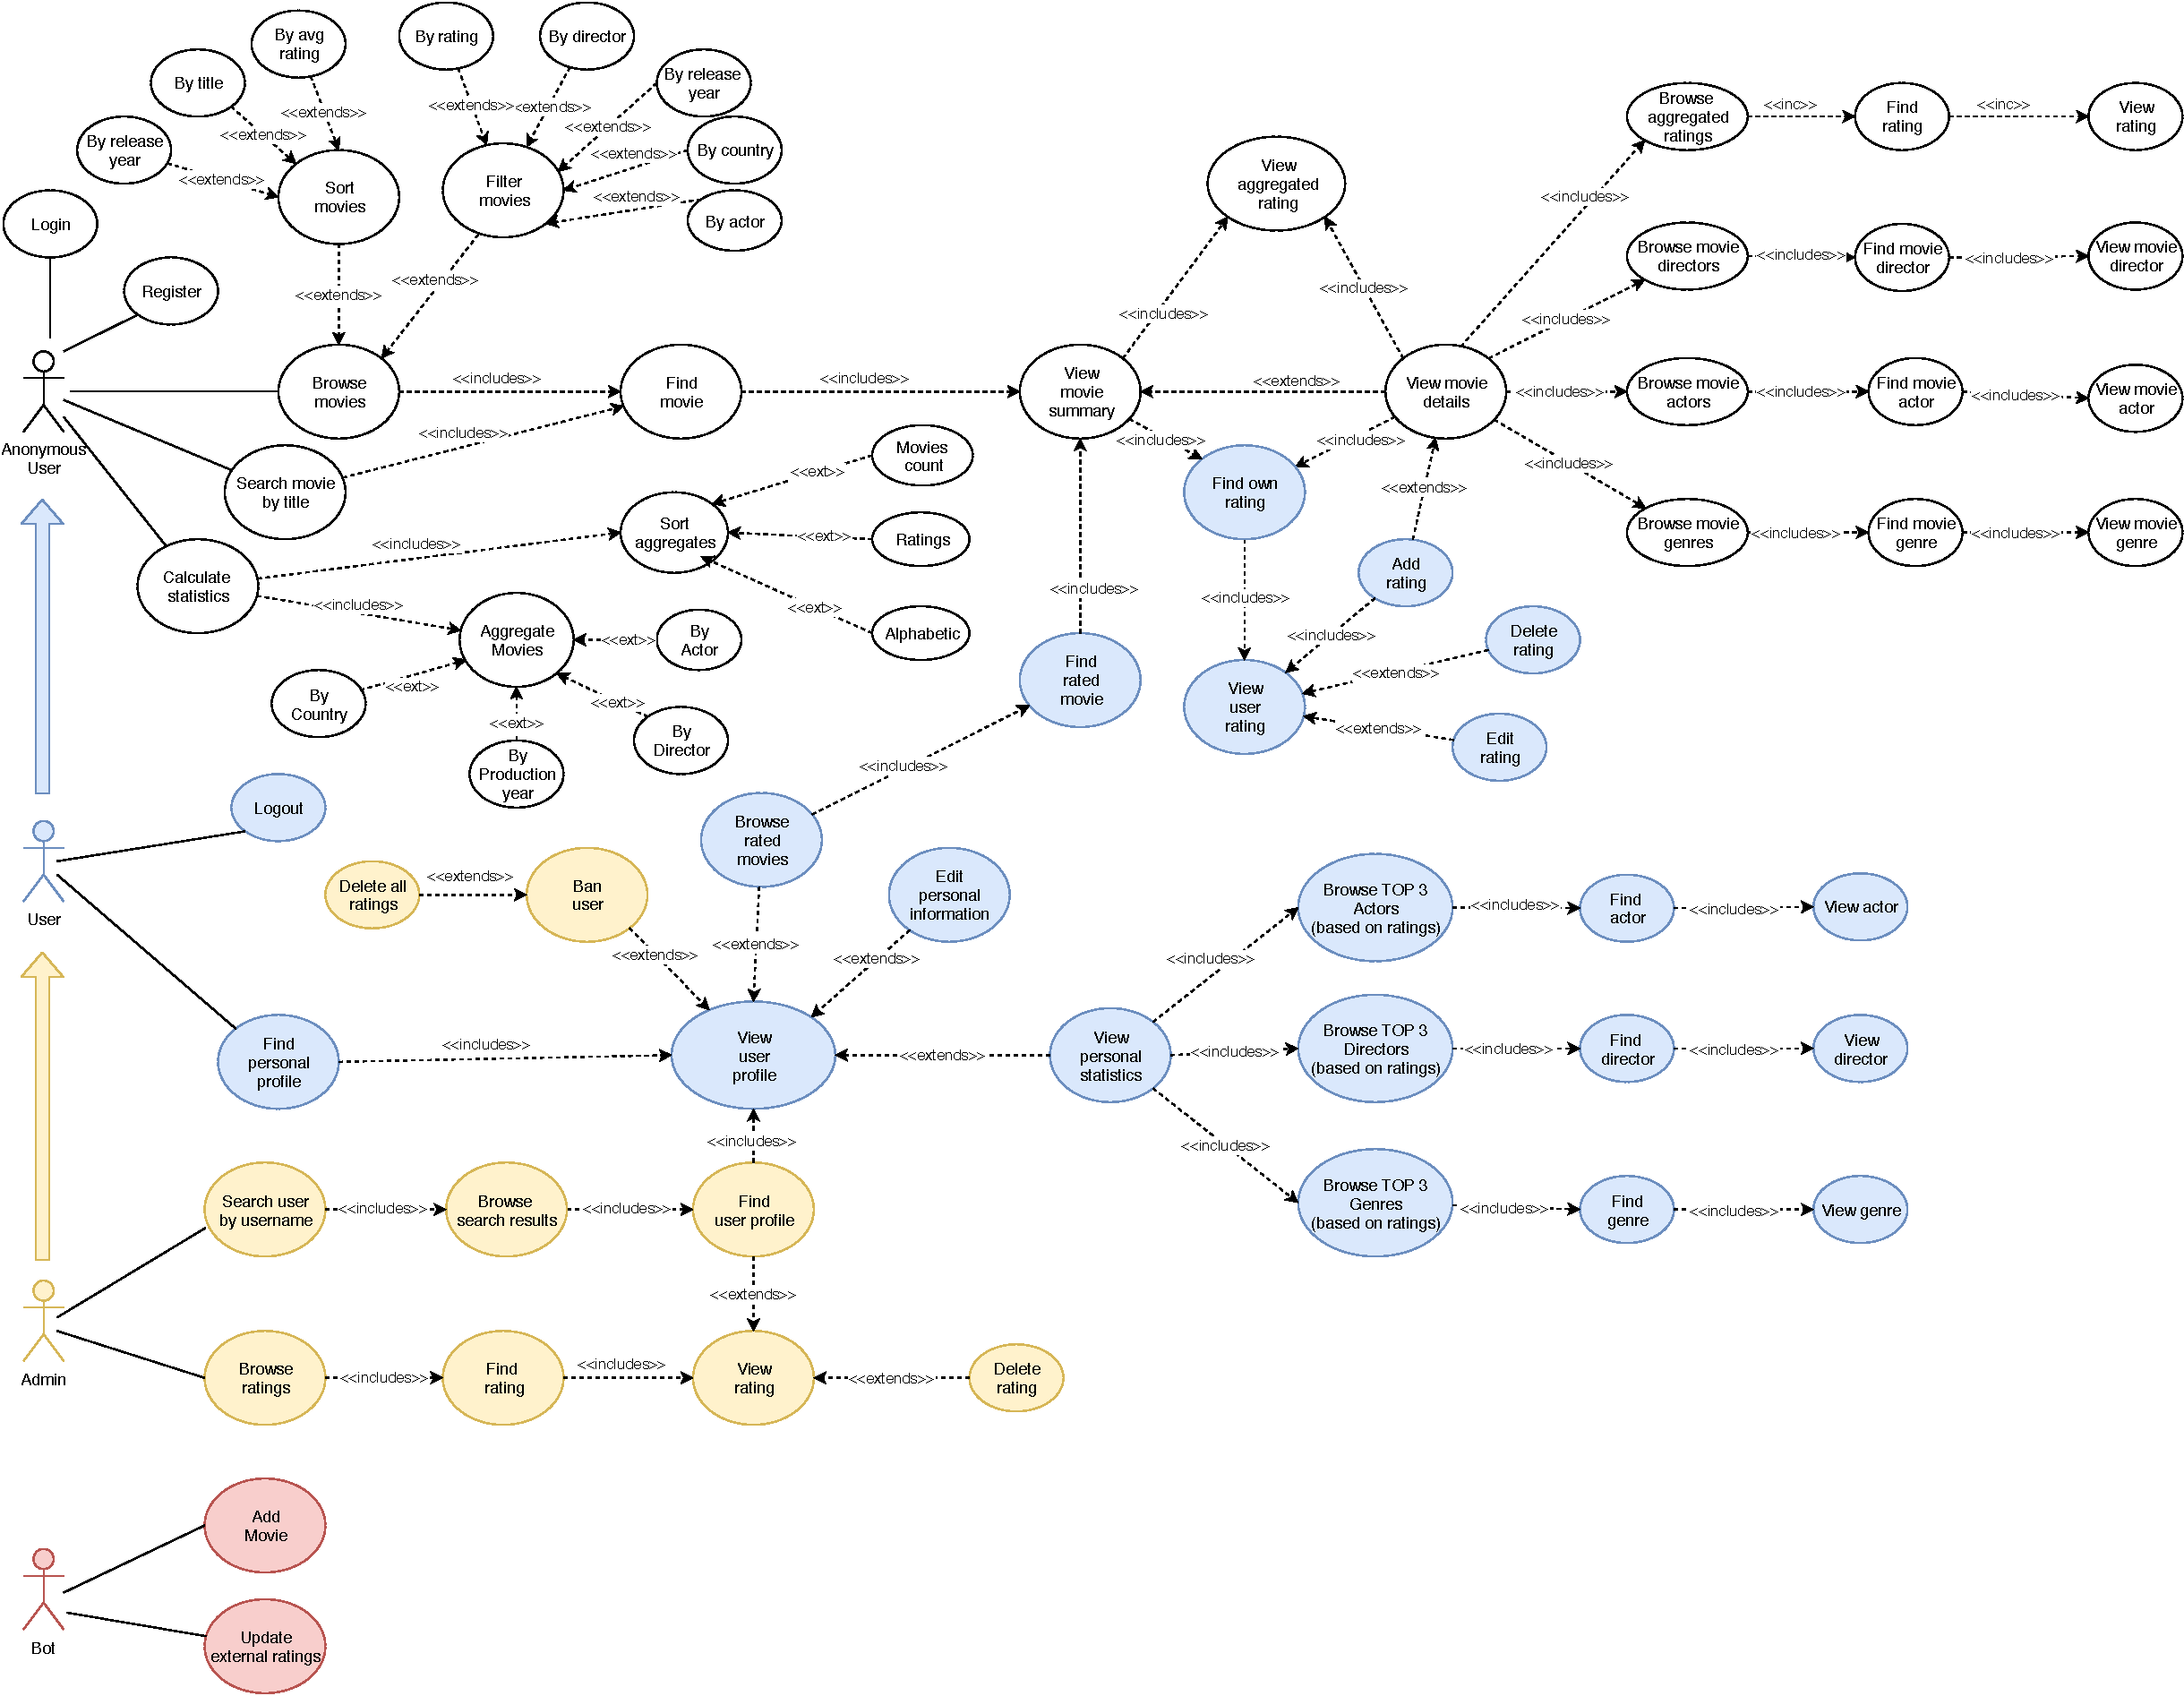
\includegraphics[height=18cm]{figs/use_case.pdf}
    \caption{Use-case diagram}
    \label{fig:usecase}
\end{sidewaysfigure}

The use-case diagram is shown in \cref{fig:usecase}. Different colors are used to highlight cases that are exclusive of some actors: white cases are referred to all users; blue cases are referred to registered user and admin; yellow cases are exclusive of the admin.

\subsection{Class diagram}

\begin{figure}[h!]
    \centering
    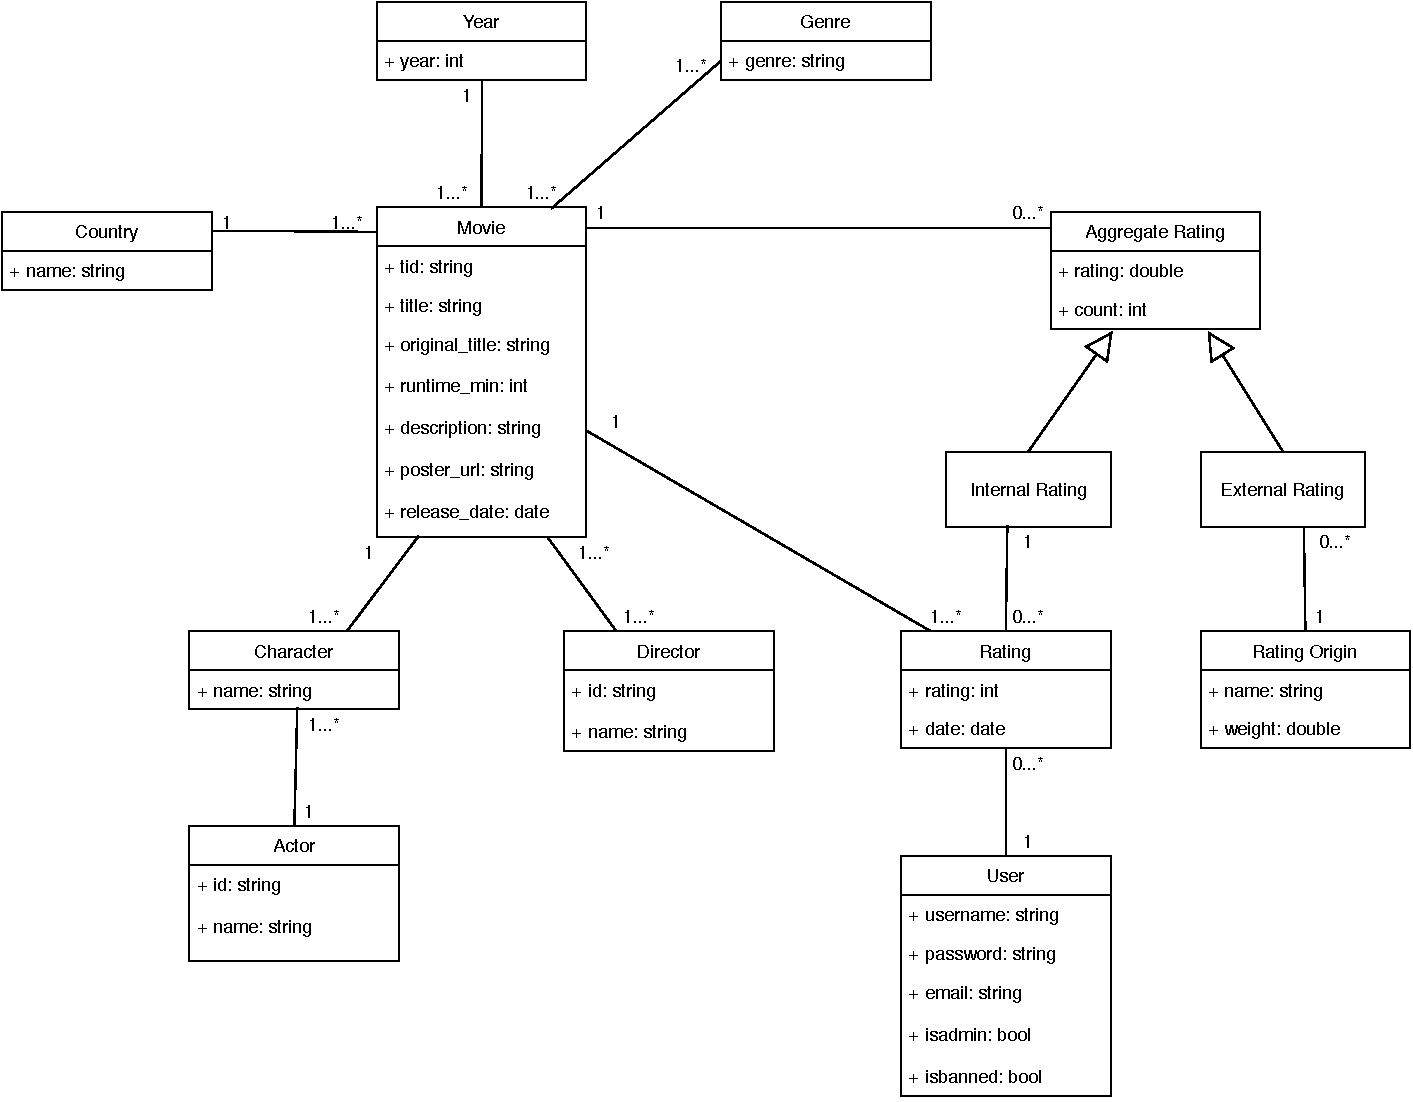
\includegraphics[width=\textwidth]{figs/class_diagram.pdf}
    \caption{Class diagram for the identified entities}
    \label{fig:class_diagram}
\end{figure}

The class diagram is shown in \cref{fig:class_diagram}. It was decided to show \emph{Country}, \emph{Year} and \emph{Genre} as separate entities as they are some of the fields over which aggregate statistics are calculated.

% ------------------------------------------------------------------------------

\clearpage
\subsection{Data model}
The data model is split in 3 different collections:
\begin{itemize}
	\item Movies (\cref{sec:movies})
	\item Users (\cref{sec:users})
	\item Ratings (\cref{sec:ratings})
\end{itemize}
In each following subsection, an example document is shown for every collection.

\subsubsection{Movies}
\label{sec:movies}

\begin{lstlisting}[language=json]	
{
	"_id": "tt7286456",
	"title": "Joker",
	"original_title": "Joker",
	"runtime": 122,
	"countries": ["USA", "Canada"],
	"original_language": "English",
	"year": 2019,
	"date": "2019-10-04",
	"description": "In Gotham City, mentally troubled comedian [...]",
	"storyline": "Joker centers around an origin of the iconic arch [...]",
	"tagline": "Put on a happy face.",
	"poster": "https://m.media-amazon.com/images/M/[...].jpg",
	"mpaa": "Rated R for strong bloody violence, disturbing behavior, [...]",
	"budget": 55000000,
	"gross": 1074251311, 
	"characters": [
		{
			"name": "Joker",
			"actor_name": "Joaquin Phoenix",
			"actor_id": "nm0001618"
		},
		...
	],
	"directors": [
		{
			"id": "nm0680846",
			"name": "Todd Phillips",
		}
	],
	"genres": ["Crime", "Drama", "Thriller"],
	"ratings": [
		{
			"source": "internal",
			"avgrating": 9,
			"count": 100,
			"weight": 2,
			"last_update": "2019-11-28 12:34:56"
		},
		{
			"source": "IMDb",
			"avgrating": 8.6,
			"count": 628981,
			"weight": 1,
			"last_update": "2019-11-28 12:34:56"
		},
		...
	],
	"total_rating": 8.87,
	"last_scraped": "2019-11-28 12:34:56"
}
\end{lstlisting}

\paragraph{Notes}
Character and director nested documents contain redoundant data (person's name) that is introduced to reduce the number of seeks necessary to return the movie details
to the user.

This collection is mainly read-heavy since most fields will be written only once.
The only fields subject to change are the ones related to ratings. For these reasons,
we can affort many indices to speed-up the aggregations.

\paragraph{Indices} 
Indices on the following fields will be set for this collection:
\begin{itemize}
	\item \texttt{title}: speed-up sorting by title
	\item \texttt{title}, \texttt{original\_title} (text\ index): movie lookup 
			by name
	\item \texttt{countries} (multikey index): filter and aggregation by country
	\item \texttt{genres} (multikey index): filter and aggregation by genre
	\item \texttt{year}: filter and aggregation by year
	\item \texttt{characters.actor\_id} (multikey index): filter and aggregation by actor
	\item \texttt{directors.id} (multikey index): filter and aggregation by director
	\item \texttt{total\_rating}: filter and sorting by rating
	\item \texttt{last\_scraped}: fast lookup for next-to-be-scraped movie (oldest movie).
\end{itemize}

Among this fields, \emph{total\_rating} is the only one that will be updated 
frequently (all other fields with index are updated with the periodic scraper 
whose period is of some days). However it is necessary to efficiently fulfill 
many queries.

\subsubsection{Ratings}
\label{sec:ratings}

\begin{lstlisting}[language=json]	
{
	"_id": {
		"user_id": <ObjectId>,
		"movie_id": "tt7286456"
	},
	"date": "2020-01-20",
	"rating": 10
}
\end{lstlisting}

\paragraph{Notes}
The raw ratings are kept separated from the movie they refer for three reasons:
\begin{enumerate}
	\item single ratings are never shown to the user, except when the user 
			looks his own ratings or when the admin looks all ratings	
	\item they may be accessed per-user, per-movie (for calculating 	
			statistics) and globally (by the administrator). The optimization for one use-case would influence the performance of another.
	\item new ratings are expected to be frequently added and, thus, the use of 
		a nested document inside the \emph{movies} collection would be 
		infeasible beacause it would grow indefinitely. 
\end{enumerate} 

However, this choice mandates the introduction of indices for efficiently 
obtaining ratings of a user or ratings of a movies are required.

\paragraph{Indices} 
\begin{itemize}
	\item \texttt{\_id.movie\_id}: speed up aggregations on movie.
	\item \texttt{\_id.user\_id}: speed up user ratings browse.
	\item \texttt{date}: speed up browsing user and global ratings.
\end{itemize}

\subsubsection{Users}
\label{sec:users}

\begin{lstlisting}[language=json]	
{
	"_id": <ObjectId>,
	"username": "joker",
	"password": "<HASHED PASSWORD>",
	"email": "joker@dccomics.com",
	"isadmin": True (optional),
	"isbanned": False (optional),
	"sessions": [
		{
			"session_id": "<session_id>",
			"expiry": "2020-01-28"
		},
		...
	]
}
\end{lstlisting}
\paragraph{Notes}
\emph{Username}, \emph{email} and \emph{session\_id} must be unique across the whole collection.

\paragraph{Indices} 
\begin{itemize}
	\item \texttt{username} (text index): find user by username
	\item \texttt{username}: find user by exact username
	\item \texttt{email}: find user by email
	\item \texttt{sessions.session\_id} (multikey index): find user by session id
\end{itemize}

\subsection{Software Architecture}

The application will be made of the following 4 components:
\begin{itemize}
	\item \textbf{Mongo DB}: a MongoDB cluster will be deployed with
		replication.
	\item \textbf{React Frontend}: web-based UI.
	\item \textbf{Java Backend}: using \emph{Spring}, the \emph{Java backend} will provide REST APIs to the \emph{React frontent}.
	\item \textbf{Updater ``bot''}: two Python scripts are needed in order to nightly update the DB with the latest movies and ratings: 
	\begin{enumerate}
		\item the \textbf{IMDB parser} periodically parses the IMDb dataset to add the latest movies.
		\item the \textbf{scraper} continuously parses the rating sources to update the ratings.
	\end{enumerate}
	These scripts will executes asynchronously from the \emph{Java backend}.
\end{itemize}

% ------------------------------------------------------------------------------

\section{Database}

\subsection{Creation of the database}
The database is created from scratch starting from the public IMDb dataset available at the link \href{https://www.imdb.com/interfaces/}{https://www.imdb.com/interfaces/}.

We developed a Python script, in order to obtain the data in the form described in the Data Model. However, some information where missing. So we integrated missing information scraping them from other movie's sites while we were scraping for ratings.

Collections are saved into Json files and then upserted in MongoDB database with another simple python script with the use of the \textbf{UpdateOne} module. Update requests are inserted in append into an array and served through the \textbf{bulk\_write()} function.

\subsection{Scraping}

\subsection{Updating the database}

% ------------------------------------------------------------------------------

\section{Backend Implementation}
The API specification can be found in the \texttt{docs/api.md} file. This section will go through the implementation of the main APIs. 

\subsection{Java classes overview}
TODO
 - Class diagram
 - Some words
 - Each class has an Adapter to conveniently convert from/to Mongo Document

\subsection{Authentication}

\paragraph{Register}
In order to register a user, it must first be checked that no user with same username and password exists (snippet 1) and then, if no duplicate entry is found, the user can be added to the database (snippet 2). If creation was successful, a new session for the new user is then added (snippet 5). Any subsequent API call must be accompanied by the session identifier in order to identify the user (snippet 6).

\paragraph{Change Password}
This query (snippet 3) is simply done by matching the user by username and setting the new password.

\paragraph{Login}
In order to authenticate the user, a matching user with same username and password is found in the database (snippet 4). If a user matches, a new session
for the given user is then added (snippet 5).

\paragraph{Logout}
The session is removed from the DB (snippet 7).

\lstinputlisting[language=Java]{figs/code/authentication.java}

\subsection{Movies}
\subsubsection{Browse}
Returns a list of filtered movies with the given sorting. The result is paged.

\begin{enumerate}
	\item build a list of filters based on user specifications. People names are
			matched if all words in the query sring are substrings of the full 
			name (this is done using a regex).
	\item Make the filter to pass to the \emph{find} function by and-ing all 
			conditions.
	\item Make the query:
		\begin{description}
			\item[find] all movies matching the conditions
			\item[sort] by the user-defined sort order
			\item[project] only movie important details
			\item[skip] the first \emph{n} pages
			\item[limit] the results to the page size
		\end{description}
\end{enumerate}

If user is logged in, a separate query will be done to fetch the user's ratings of the returned movies (\ref{sssec:userratings}).

\lstinputlisting[language=Java]{figs/code/browse_movies.java}

\subsubsection{Search}
During a search, movies that (fuzzy) match the entire query are returned sorted
by ``likelyhood'' (meta text score, in MongoDB). Results are paged as before.

If user is logged in, a separate query will be done to fetch the user's ratings of the returned movies (refer to \ref{sssec:userratings}).

\lstinputlisting[language=Java]{figs/code/search_movie.java}

\subsubsection{Get Details}
Given a movie id, return all movie details. Code snippet not reported for brevity's sake.

\subsubsection{Browse Statistics}
This function is used to return aggregated statistics on movies based on one of the following information attributes:
\begin{itemize}
	\item genre
	\item year
	\item country
	\item director
	\item character
\end{itemize}
Before performing the aggregation, movies can be filtered as shown in the \textit{GetMovieList} API.
The statistics returned show the following informations about the aggregation attribute:
\begin{itemize}
	\item aggregated attribute
	\item average rating calculated on the aggregation
	\item number of movies present in the aggregation (calculated after filtering)
\end{itemize}
Results can also be sorted in ascending or descending order based on each of the previous attributes.

The aggregation pipeline is performed with the following code:

\lstinputlisting[language=Java]{figs/code/aggregation.java}

The \textbf{match} function uses the array of conditions "\textit{filters}" to perform all the filters in a single step. \textbf{Unwind} deconstructs the array field and returns a document for each array element (this is necessary for country, director and character fields). Then, the \textbf{group} function groups documents by the value expressed in the "\textit{realGroupBy}" and then applies accumulator expression to each group:
\begin{itemize}
	\item \textbf{Accumulators.first} sets "\textit{realGroupName}" as name of the group
	\item \textbf{Accumulators.avg} calculates the average rating of all the "\textit{total\_rating}" and saves them in the "\textit{avg\_rating}" attribute
	\item \textbf{Accumulators.sum} calculates the number of movies in the aggregation, by adding 1 to the variable "\textit{movie\_count}" for each movie
\end{itemize}
After that, the results are sorted with the \textbf{sort} function, where the argument "\textit{sorting}" is calculated as follow:

\lstinputlisting[language=Java]{figs/code/sorting.java}

Here, "\textit{realSortBy}" is the value to sort.

Finally, the \textbf{skip} and the \textbf{limit} functions are used to manage the display of the results.
%scrivere qualcosa sul ritorno?

\subsection{Ratings}
\subsubsection{CRUD operations}
A rating can be added, read, updated or deleted. Related code snippets are not shown for brevity's sake.

After a rating is updated, the corresponding movie rating information are asynchronously updated (refer to \ref{sssec:updateInternalRating}).

\subsubsection{Get all ratings for a user and list of movies}
\label{sssec:userratings}
This particular operation is done to add the user's ratings to a query result set. First the list of movie ids of the movies in the query result is built and then all ratings of the given user to any of those movies is returned.

By building the array of identifiers, just one query to the database is necessary.

\textbf{NB}: the number of movies will always be small due to paging (20).

\lstinputlisting[language=Java]{figs/code/fill_user_ratings.java}

\subsubsection{Browse All}
Admins can browse all ratings in the collection in descendig date order. Results are paged as seen in previous sections. Related code snippet is not shown for brevity's sake.

\subsubsection{Browse User Ratings}
Users can browse all their ratings in descendig date order. Results are paged as seen in previous sections. Related code snippet is not shown for brevity's sake.

\subsubsection{Update Internal Rating}
\label{sssec:updateInternalRating}
After a rating is changed, the average internal rating and the total rating of the movie should be updated. This is done asynchronously after the update in order not to make the client wait for this additional operation.

The update takes in input the old and the new rating (one of them can be null in case of insertion or delition) and consists in three parts:
\begin{enumerate}
	\item fetch the movie from the DB
	\item calculate new statistics
	\item update the database. Both internal rating and total rating are updated. For the former there are three cases:
	\begin{itemize}
		\item the internal rating was not present before and it needs to be added.
		\item the internal rating existed and needs to be updated
		\item the internal rating existed and needs to be removed
	\end{itemize}
	For the total rating there are two cases: update or unset in case the rating we removed was the last one.		
\end{enumerate}

Furthermore, this operation is also protected from possible concurrent bakends running in other machines since it modifies the database only if it detected no updated between the fetch of the movie and the updated. It does so by making sure that the \emph{last\_updated} field remains the same by adding a filter in the update query (if no internal rating was present before it just checks that it was not added in the meanwhile). In case of failure, it retries up to 5 times. It is very unlikely to fail but in case it will be corrected by the scraper that always builds the internal rating using the Ratings collection.

\lstinputlisting[language=Java]{figs/code/update_internal_rating.java}

\subsection{Users}
\subsubsection{Get Profile}

\subsubsection{Ban}

\subsubsection{Search}

\section{Replication}
\subsection{Configuration of the replica set}
Replication has been achieved through the set up of a MongoDB replica set in a remote cluster of 3 virtual machines provided by the University of Pisa.

A configuration document has been written, specifying the id of the replica set and the addresses of the machines. Additionally, a location tag was included. This could be useful if, in the future, the application is deployed to multiple datacenters for a more fine-grained control over the database requests (e.g. writes could be applied to at least one machine in every datacenter before returning ). 

\begin{lstlisting}[language=json]	
rsconf = {
	_id: "replicaset0",
	members: [
	{_id: 0, host: "172.16.1.251:27017", tags: { location: 'unipi'} },
	{_id: 0, host: "172.16.1.162:27017", tags: { location: 'unipi'} },
	{_id: 0, host: "172.16.1.195:27017", tags: { location: 'unipi'} }
	]
}
\end{lstlisting}

By default MongoDB binds only to localhost, to allow connection through the network the \lstinline{mongod} daemon was started with the \lstinline{--bind_ip} flag.

\begin{lstlisting}[language=bash]
mongod 	--replSet replicaset0
		--dbpath ~/data/rs_db
		--oplogSize 200 
		--bind_ip 172.16.1.162
\end{lstlisting}
\subsection{Authentication}
\subsection{Consistency, Availability and Partition tolerance}
The CAP theorem states that only two between consistency, availability and partition tolerance could be achieved in a database: our main service, providning movies infos and ratings, could work well even if with outdated data.
Movie's description or title rarely chages while ratings should have a low variability: it is therefore the most convenient choise to increase our availability and partition tolerance.
This is not true for what concerns logins and accounts in general: e.g a password change should be set in stone or the user creation should grant login consistency. A bad user experience is the consequence of not handling correctly this aspects.

Different handling of the write and read requests depending on the data we want could be a reasonable solution.
The drivers connecting to the database can specify a WriteConcern and a ReadPreference: the first determines the number of members of the replica set that should have written the new data before a positive response is sent to the driver, the second option is about the possibility of reading from nodes other than the master.
The default configuration of MongoDB is a WriteConcern equal to 1 (only the primary server is updated) and a ReadPreference of 'primary' (we can read only from the primary). This means that, in case of a network partition excluding a number of nodes less than the majority and including the master, thus with the election of a new primary, consistency is not guaranteed since a write could have been made just before the partitioning (and the read would work just fine from the newly elected master).

What has been chosen, as already anticipated, is a differentiated approach depending on the request. To access the \lstinline{users} collection, the driver establishes three different connections with the database.

\begin{lstlisting}[language=java]
mongoClient = MongoClients.create(connectionURI);
database = mongoClient.getDatabase(dbName);

moviesCollection = database.getCollection("movies").withReadPreference(ReadPreference.nearest());

usersCollection = database.getCollection("users").withReadPreference(ReadPreference.nearest());

usersCollectionMajorityWrite = database.getCollection("users").withWriteConcern(WriteConcern.MAJORITY);

usersCollectionPrimaryRead = database.getCollection("users").withReadPreference(ReadPreference.primary());

ratingsCollection = database.getCollection("ratings").withReadPreference(ReadPreference.nearest());
\end{lstlisting}

\lstinline{usersCollection} will be used for all the requests where we want high availabillity, like showing up the profile page or finding the user from the admin control page.
\\
\lstinline{usersCollectionMajorityWrite} handles all the requests for which we want the updates to be permanent (e.g. password changes, new session id etc.): a write concern of 'majority' (which is computed against the total nodes in the replica set) protects us against network partition since no matter what happens to the nodes, as long as a majority is reached, the election system will make sure the successive primary node will have our write. Since the secondaries could or could not have it, when we want consistency we have to read only from the primary. Therefore, the \lstinline{usersCollectionPrimaryRead} will set the correct ReadPreference and will be used accordingly.

For what concerns the other requests, consistency is not strictly necessary and we would like our system to be highly available. For this reason, we keep the default write concern (equal to 1) and set the read preference to 'nearest', thus allowing reads from secondaries (which could have outdated informations).
\end{document}